\chapter{関連研究}\label{chap:related}

本章では、関連研究、及び本論文に関連する先行サービスについて紹介する。
初めに近接情報の検出に関するもの、
続いてその場の情報共有に関するものを紹介する。
最後にこれらを踏まえた本研究との比較について述べる。

\newpage

\section{近接情報の検出に関するもの}

はじめに、Context-basedなサービスに関する先行サービスおよび関連研究について紹介する。

Google Latitude\cite{latitude}は、Googleが提供するGoogle Mapsの機能として使用することのできた位置情報サービス。
Google Maps上で有効にしておくと、友達や家族など、共有を設定したユーザーと互いの現在位置をGoogle Maps上で共有できる。
2013年8月9日にサービスを終了している。

FourSquare\cite{foursquare}は、GPSによる居場所の特定とチェックインと呼ばれるユーザの来訪履歴を組み合わせたサービス・アプリケーション。
サービス上で登録しておいた友人が近くの登録された施設にチェックインをすると、情報をプッシュ通知を受け取ることが可能になる。
また、近くに友人が来訪した履歴のある施設があると、これもプッシュ通知として表示される。

\cite{槙島量:2010-03-08}は、リアルタイム性のある地域情報をデバイスに対してPush通知するシステムを提案した。
本提案では、地域を50mの矩形に分割することで、その地域の情報を通知できる他、
同矩形範囲内のユーザからも情報を引き出すことで、ユーザ同士のリアルタイムなコミュニケーションを実現している。

Bluetoothの近接検出に関して、Davidrajuh\cite{Davidrajuh:2009:EPB:1523492.1523495}らは、
マスタデバイスとPico-net上の2つのスレーブデバイスでプロトタイプを作り、
大きなサイズの教室内でのBluetooth無線技術によるScatter-net環境が有用であることを示した。

DroidSensor/すれちがったー\cite{すれちがったー}は、2009年から2010年にかけて配布されていたBluetoothとTwitterを使った、すれちがい通信アプリケーション。
すれちがったーをインストールしたデバイスが同じくインストールされた他のデバイスとすれちがうと相手のtwitter IDを呟く。
他のデバイスがすれちがったBluetoothデバイスとすれちがうと、以前にそのデバイスとすれちがった相手のtwitter IDを呟く。
どのデバイスとすれちがったかをトラッキングすることで、twitter IDを持つ本人を特定できてしまうというセキュリティの問題が議論された。


% 画像

\section{その場の情報共有に関するもの}

\subsection{Firechat}

Firechat\cite{firechat}は、OpenGardenによるApple iOSとGoogle Android向けのチャットコミュニケーションアプリ。

登録された人間同士のチャット機能の他に「周辺」というチャットルーム機能を持つ。
モバイルデバイス同士がメッシュネットワークを築くことによりインターネット接続が無くてもチャット通信が可能。
メッシュネットワークを数珠つなぎのように延ばすことで、最大70mまでのホッピングを可能としている。
Bluetooth検出のホッピングにより、最大で70mまでのデバイス検出を可能としている。

また、同様の機能を持ったアプリケーションに、2007年にはBluetoothを利用して近場のデバイス同士でチャットを行うBlueeee!\cite{Blueeee}がある。


\subsection{ライブ情報共有のためのすれちがい通信アプリ}

藤田ら、\cite{藤田大樹:2012-09-04}\cite{藤田大樹:2013-08-20}\cite{藤田大樹:2013-03-06}は、
iOS上で動作する,アドホックネットワークを用いて周囲とライブ情報を共有するためのプロトタイプLNSを実装した。
本研究はすれ違い通信\cite{菊池大輝:2012-09-04}によってライブ情報を適切な範囲に対して拡散させるためのシステムを
提案しており、共有するメッセージの有効時間とホップ数を適切に設定することで、メッセージの到達可能範囲を
発信者の近隣のみに限定した上、有効時間が切れたメッセージを自動で削除することが可能だと述べている。

\begin{figure}[h]
  \begin{center}
    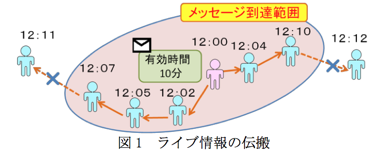
\includegraphics[width=0.5\linewidth]{img/live.eps}
  \end{center}
  \caption{システム構成}
  \label{fig:live}
\end{figure}

\subsection{Sonoba.org}

山本らは、情報をその場に居る人達に共有する手法としてSonoba.org\cite{山本伶:2013-03-06}を提案した。
本研究では、たまたま居合わせただけのような、
よく知らない相手とのその場限りの関係においてもデジタルな情報の共有をする方法として、
時限URLを用いた手法を提案し、Sonoba.orgとして実装した。
この提案では、誰もが普段持ち歩いているモバイルデバイスから共有する情報にアクセスするため、
覚えやすい文字列と、時限式で消去されるURLによる共有手法を使うことにより、その場限りの共有手法を実現している。

\begin{figure}[h]
  \begin{center}
    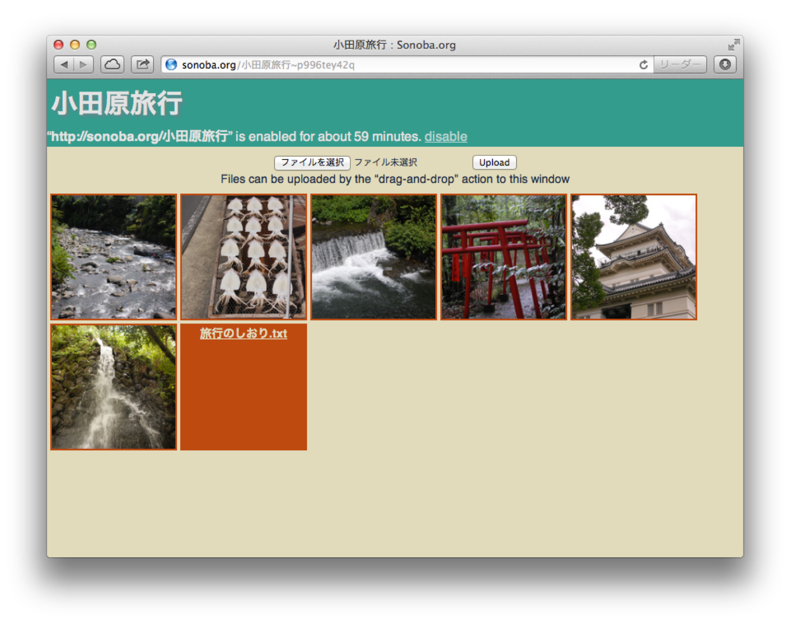
\includegraphics[width=0.7\linewidth]{img/sonoba.eps}
  \end{center}
  \caption{システム構成}
  \label{fig:sonoba}
\end{figure}

\subsection{Encore}

Adityaらは、イベント参加者の間でコミュニケーションと共有を可能にするアプリケーション、Encoreを提案した。\cite{Aditya:2014:EPC:2594368.2594374}
2つのデバイスがBluetoothの無線範囲内に存在するとき、デバイスは共有鍵を生成した上で、Bluetooth無線による通信を行う。
また、このシステムの共有鍵については、Manweilerら\cite{Manweiler:2009:SET:1653662.1653692}によれば、
デバイス感の共有鍵の交換によって、悪意のある接続から守ることが可能であると述べている。



\section{関連研究と本研究との比較}

本研究は、Sonoba.org\cite{山本伶:2013-03-06}と、近接情報の検出の文脈を受け継いでいる。
その場に居合わせた人間同士で自動的に共有のための場が作られる手法として、
近接しているというコンテキストを利用するのは強力であると言える。
それに加え、Webを介した情報共有の利便性と、情報の継続性も持つことができた。

URLの共有によってWeb上での情報共有を図る手段に比べると、
どうしてもアプリケーションのインストールという手間がある。

また、Bluetoothにおけるセキュリティとプライバシーの問題を隠匿して吸収するために、
本システムではほとんどの情報処理をサーバ側で担っている。
この構造は、ユーザが増加した時にサーバ管理のコスト増大があることは明確であり、
より低コストな構造の検討が求められる。
